\chapter{Proposed approach}
\label{chap:proposed_approach}
	\textit{This chapter displays the problems as well as the malicious request validator's input and output. Then we offer the design and architecture of the problem's solutions.}
\minitoc

WAFs, as previously indicated, are frequently used, however they suffer from high FP. Our aim is to enhance the accuracy of WAFs, using the help of machine learning rather than the rule-based approachs.  \\
Because WAFs only cover the Application Layer, the network requests are the model's input (mostly HTTP requests). Our methodology produces the same result as WAFs: whether the request is malicious or not.\\
With its nature, WAF is obligated to have fast processing speed in deciding whether an incoming request is reliable or not. For user experiences, we can't examine the request's veracity for minutes before granting or denying access. Our system's time constraint must be in milliseconds.\\
\section{API security problems}
\label{API problems}
Here are the most common vulnerabilities \footnote{Vaadata.\textit{How to strengthen the security of your APIs to counter the most common attacks?}. April 2022.
\url{https://www.vaadata.com/blog/how-to-strengthen-the-security-of-your-apis-to-counter-the-most-common-attacks/}}:
\begin{itemize}
    \item \textbf{Lack of rate limiting, DoS and brute force attacks on APIs}
    \begin{itemize}
        \item \textit{Principle and functioning of DoS attacks}
        \newline
        An assault known as \textbf{a denial of service (DoS)} aims to render services unavailable. In fact, a DoS attack functions by depleting a resource that an API requires to respond to valid requests. By overloading an API with erroneous requests, its resources are only able to reply to the ones that were submitted.

        The objective of DoS attacks is not to alter, delete or steal data. The aim is simply to damage the operation of a web service or the reputation of a company offering such services.

        It is obvious that slowing down or even blocking their services for a few minutes could lead to significant financial losses and alter users’ trust. It is therefore necessary to find solutions to protect against this, including request verification, traffic monitoring, the implementation of rules and rate limiting, etc. Similarly, during an API or web application pentest, DoS tests should be included to assess the resistance of the services to this type of attack.
        \item \textit{Brute force attacks on APIs}
        \newline
        In a brute force attack, an attacker use tools to send a steady stream of requests to an application or API in an effort to try every combination of a parameter in the hopes of making the right guesses. The goals can vary: brute-forcing an authentication form to steal an account, brute-forcing a login to retrieve private information, etc.

        This is a “trivial” attack method, easy to perform, but still very effective and widely used by attackers.
        \item \textit{Implement rate limiting mechanisms to counter DoS and brute force attacks}
        \newline
        Securing APIs against DoS or brute force attacks requires the implementation of rate limiting mechanisms. These mechanisms protect APIs and other services from excessive and abusive use, in order to ensure their availability.

        Rate restriction works on a pretty straightforward principle. It entails making requests in advance of when one or more clients—systems—might utilize more than their "fair" share of a resource. Additionally, one can lessen the danger of DoS or brute force attacks by restricting the number of requests that a specific user is permitted to send in a given window of time.

        For example, after a user has been authenticated, your API or application may apply quotas that restrict what they are allowed to do, including the limit of requests they can send.  For example, you can limit each user to a certain number of API requests per hour, to prevent them from flooding the system with too many requests.

        Similar to this, you can set limitations before authenticating a user to lower the overall number of requests, or just those coming from a specific IP address or time period. Therefore, if rate limitation is enabled, your API will monitor the volume of requests and reject those that are greater than the permitted threshold. Additionally, rules can be applied to totally shut off connections when the limit is reached or to sluggish down request processing. This action is referred to as "throttling."
        
        In short, Rate Limiting prevents resource depletion by managing rules and quotas.  There are different techniques for applying rate limiting, each with its own specificities: Token bucket, Leaky bucket, Fixed window and Sliding window.
    \end{itemize}
    \item \textbf{Lack of user input validation and injection attacks}
    \begin{itemize}
        \item \textit{Code injections}
        \newline
        Code injection is one of the most common types of injection attacks. If attackers know the programming language used by an application or API, they can inject code through text input fields to force the web server to execute the desired instructions.
        \item \textit{SQL injections (SQLi)}
        \newline
        Injections represent a significant part of the vulnerabilities encountered in applications and APIs. The best known and most dangerous is SQL injection.

        In an SQL injection attack, an attacker injects data to manipulate SQL commands, thereby interacting with the database through unintended queries. These flaws can lead to theft, deletion or manipulation of stored data. Worse still: if the rights are too permissive, this can even lead to a compromise of the server. 

        Let’s look at this in more detail with a concrete example:
        
        One can imagine an API endpoint that returns the information of a country based on its “CountryCode”.\\
        \begin{figure}[!h]
         \centering
         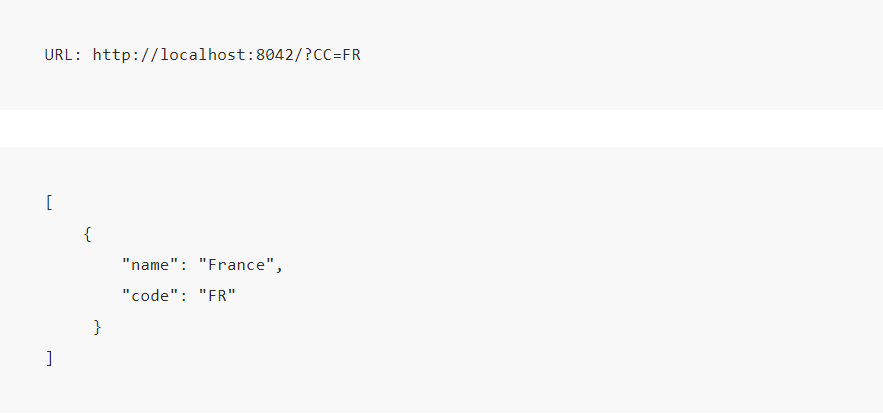
\includegraphics[width=\linewidth, height=10cm,keepaspectratio]{figures/ex1.PNG}
         \caption{Returned information}
        \end{figure}

        \newpage
        To perform the desired action, the query interacts with a database. Below is the SQL query that the server must run on the database.
        \begin{figure}[!h]
         \centering
         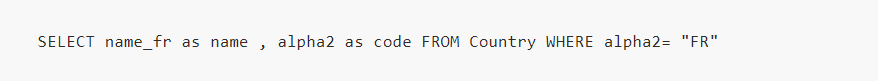
\includegraphics[width=\linewidth, height=10cm,keepaspectratio]{figures/ex2.PNG}
         \caption{Compulsory query}
        \end{figure}
        \newpage
        Example of a vulnerable PHP code:
        \begin{figure}[!h]
         \centering
         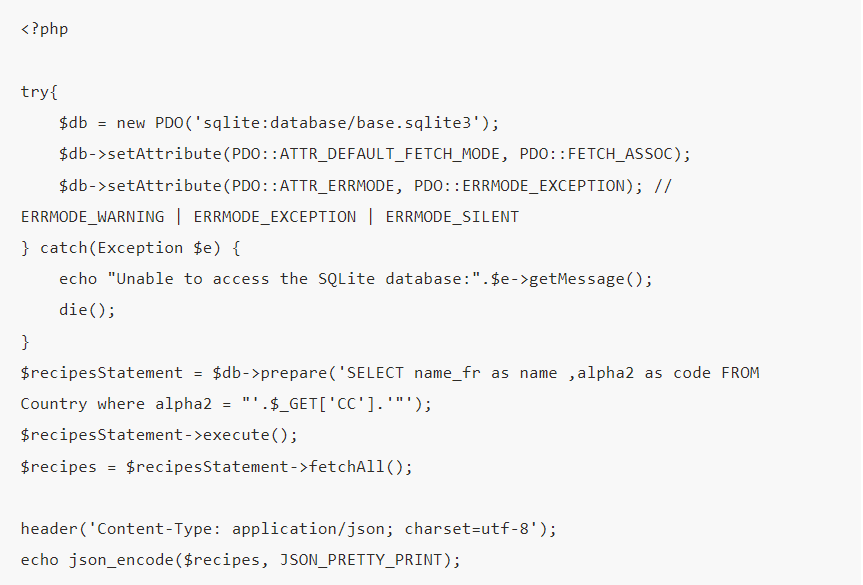
\includegraphics[width=\linewidth, height=10cm,keepaspectratio]{figures/ex3.PNG}
         \caption{Vulnerable PHP Code}
        \end{figure}
        
        As we can see, the CC parameter that is controlled by the user is directly concatenated to the query.

        Now, let’s assume that on this same database, there is a ‘users’ table that contains the email addresses and passwords of the users registered on the application. Let’s look at what happens if an attacker makes the following query:
        \begin{figure}[!h]
         \centering
         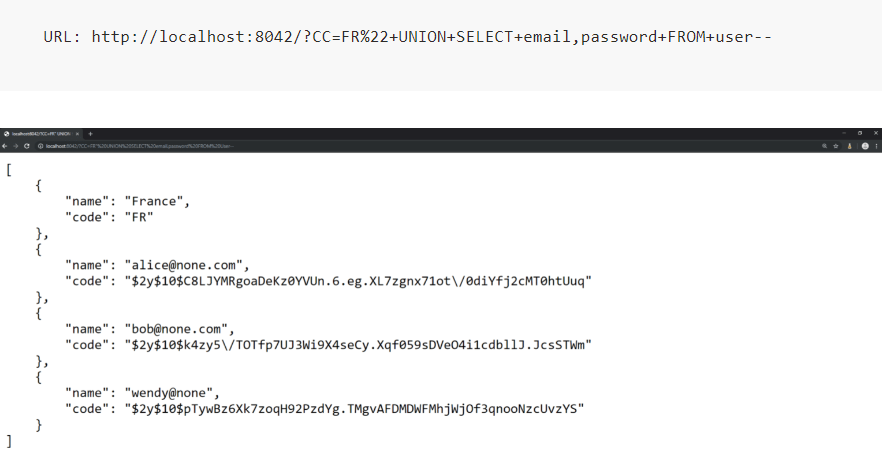
\includegraphics[width=\linewidth, height=10cm,keepaspectratio]{figures/ex4.PNG}
         \caption{The hacker's query and result}
        \end{figure}
        \newpage
        In addition to the country name, this query retrieves all users and their password hashes.

        This SQL injection flaw was discovered. A  flaw that enables an attacker to "pervert" the SQL query the program generates. The attacker may be able to view or even change the database's data with this behavior. Evidently, if an API or online application penetration test were conducted, this significant vulnerability would be discovered and disclosed.
        
        \item \textit{Validate user input to prevent injection attacks}
        \newline
        The strongest defense against SQL and code injections is validating user input. In theory, it should be recognized that data received by an application or API cannot be deemed "always" safe. In order to prevent such vulnerabilities, it is necessary to put in place methods to verify that user input meets the anticipated parameters.

        The most effective method of protecting against SQL injections is the use of prepared statements, which separate the SQL commands from the data sent by a user.

        The fix is to use prepared queries. On the PHP documentation we can see the following information:
        \begin{itemize}
            \item The query can be run multiple times with the same or different parameters after only one analysis (or preparation). The database will parse, construct, and optimize its plan to execute the query once it is prepared. If you have to repeat the same query multiple times with various parameters, this procedure can be very time-consuming for sophisticated queries, which will slow down your apps. You can avoid repeating the cycle of analysis, compilation, and optimization by using prepared statements. In short, prepared queries execute more quickly and with fewer resources.
            \item You don't need to surround query parameters in quotes; the driver takes care of it. If your application only employs prepared statements, you can be certain that SQL injection is not a possibility (however, if you build other parts of the statement based on user input, you are still taking a risk).
        \end{itemize}
        Thus, the following code is correctly protected against SQL injections:
        \begin{figure}[!h]
         \centering
         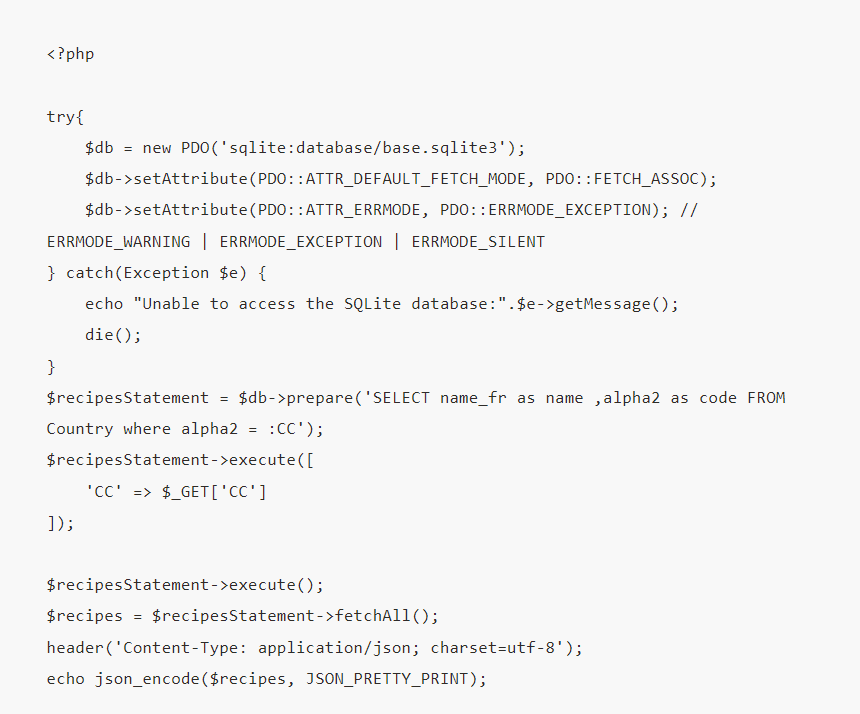
\includegraphics[width=\linewidth, height=10cm,keepaspectratio]{figures/ex5.PNG}
         \caption{The code is protected against SQL injections}
        \end{figure}
        
        As we can see, the difference with the vulnerable code is that the parameters coming from a user are no longer concatenated with the query, but directly provided at query execution. This also shows that a prepared statement can still be vulnerable to SQL injection if the data is concatenated. Because in the vulnerable example it was already a prepared statement that was used.
    \end{itemize}
    \item \textbf{Lack of data encryption and Man In The Middle attacks}
    \begin{itemize}
        \item \textit{Man In The Middle attacks}
        \newline
        An attack known as a "Man in the Middle" occurs when a hostile person intrudes on a communication or data transfer taking place between a client and a server, a server and a server, or a client and a client. Its goals might vary, from merely intercepting sensitive data—such as passwords, financial information, personal information, and sensitive documents—to manipulating communication in order to, for instance, implant malware.

        This type of attack is possible if and only if the communications are not encrypted. It is therefore quite easy to protect against it.
        \item \textit{Encrypting data with TLS to counter Man In The Middle attacks}
        \newline
        One of the most fundamental components of guaranteeing the security of an API or service is encryption. Indeed, the encryption protocol TLS (the successor to SSL) ensures safe communications over a computer network. Connections between a client and a server that are TLS-secured include one or more of the following characteristics:
        \begin{itemize}
            \item The connection is private (i.e. secure) because the data transmitted is encrypted. 
            \item The encryption keys are uniquely generated for each connection and are based on a shared secret negotiated at the beginning of the session.
            \item The connection guarantees integrity because each transmitted message includes a signature verification of the integrity of the message, thus avoiding any undetected loss or alteration of the data during transmission.
        \end{itemize}
    \end{itemize}
    The use of this encryption protocol therefore reduces or even eliminates the risks of Man In The Middle attacks. Furthermore, to reinforce security, we recommend implementing the HSTS (http Strict Transport Security) header on your servers in order to force a browser to use HTTPS secure connections. Without this setting, you run the risk of users accessing your domain without the HTTPS protocol, which can lead to a breach in communications. 
    
\end{itemize}
\section{Designs}
\label{design}
To summary, numerous strategies for identifying malicious URLs have been proposed. Most of these solutions utilize supervised-based machine learning techniques for classification. This technique can detect irregularities between requests, but it cannot extract these abnormalities into human-readable form in order to reconstruct the WAF. Relying solely on machine learning eventhough brought higher accuracy like in \cite{s22093373}, WAFs need to be time-efficient. We can not compromise accuracy for speed, hence these methods don't work for WAFs.\\
We come to the approach is to categorize the incoming request and analyze its structure, with moderate reliability, then combining the result of these two process to achieve the high precision yet does not expending an excessive amount of time
\subsection{Architecture}
\label{architecture design}
\subsubsection{Data exploration and Sanitization}
\label{data preprocessed}
Our goal is to classify request supplied as inputs in order to determine whether they are harmful or inoffensive. The sample of request data consists of different categories including: 
\begin{itemize}
    \item \emph{Plain text:} request that contains data but does not trigger any machine execution, typically in the form of HTML, JSON, XML, and CSV, etc.
    \item \emph{Client-side script:} request in form of programming languages or scripts that can be executed on client's machine
    \item \emph{Server-side script:} request in the form of programming languages (mostly back-end programming languages like PHP, JAVA, PYTHON, and so on) that can change the behavior of the application or web
    \item \emph{Shell script:} request in the form of shell scripts that can run jobs on the server or change the server's or operating system's behavior
    \item \emph{SQL script:} request that in form of SQL, can be used to query data from the database.
\end{itemize}
 The textual data acquired in the previous phase is going to be cleaned and standardized. To minimize feature complexity and improve classification performance, the request was preprocessed by eliminating symbols and punctuation. The text data collected will be transformed to lower case and then normalized. The goals of the normalization procedure were dual. First, the text must be converted from unstructured data to a structured word vector. Second, by deleting unneeded words and decreasing the number of words by roots them to their originals, we may reduce the scarcity of feature vectors.
However, malicious attacker usually use methods like slight modification to make an imposter URL or request looks legitimate, we skip severals step in conventional Natural Language Processing: 
\begin{itemize}
    \item Removing stop word
    \item Stemming (the process of reducing infected words to their stem)
    \item Lemmatization (returning to the base form of the words...)

\end{itemize}
\subsubsection{Model Selection and applying Natural language processing}
\label{NLP}
Because four of the five categories are structured languages, we must first create a special tokenizer to map the request into a defined set of keywords (client-side script, server- side script, and SQL script).
To convert the words (the tokens) to their numerical equivalents, a corpus containing a list of unique tokens based on their frequency of occurrence in each class was created. To put it in more formal mathematical terms, the TF-IDF score for the word t in the document d from the document set D is calculated as follows:
\begin{align}
    tf\:idf(t,\: d,\: D)\; =\; tf (t,\: d) \; . \; idf (t.\: D)
\end{align}
Where: 
\begin{align}
    tf(t,\: d)\; =\; 1 \: + \: log(freq(t,\: d)) \: \: \\
    idf(t, \:D)\; = \; log(\frac{N}{count (d \: \in D :t \in d)})\:  \:
\end{align}
The statistical-based text representation, TF-IDF, was then computed using the following equation: 
\begin{align}
    tf\; \_ \; idf \;=\; tf\:.\:log(\frac{N}{df})
\end{align}
 where $tf$ is the term frequency of the word in a specific instance, $df$ is the document frequency for the word, $N$ is the number of samples in the dataset. The term frequency $tf$ is the number of times a word has occurred in the sample while the inverse document frequency $idf$ refers to the inverse number of documents where the word has occurred. The higher the $tf \_ idf$ of a word in a document, the more relevant the document. The output of this phase was three numerical vectors for each sample.
\subsubsection{Distinguishing request }
\label{distinguishing request}
We present a hypothesis: all normal server requests fall into the same category. A static web request, for example, may only contain plain text, whereas API server requests are mostly in JSON format, incoming database queries are SQL, and online compilers use programming language-format requests. A malicious request must be classified differently than normal requests, such as a script request to a static web server or API server, which can be classified as code injection \footnote{Code injection is the exploitation of a computer bug that is caused by processing invalid data. The Injection is used by an attacker to introduce code into a vulnerable computer program and change the course of execution.}  or command injection \footnote{Command injection is an attack in which the goal is the execution of arbitrary commands on the host operating system via a vulnerable application.}. SQL requests to an API server can be classified as SQLi, and script requests to a database can be classified as command injection or stored XSS attacks. We can determine whether a request is 'normal' to a server by comparing the types of incoming sketchy requests to the average categories of normal requests. If the similarity is low, we can consider that the origin of the incoming request is unusual. For example, if a typical request to a secured server is in JSON format (plain text), but a suspicious request is in JavaScript (client-side script), we can conclude that the incoming request is malicious. If a suspicious request is in XML format (plain text), we can safely assume that the user made a mistake and the alert was false.\newline
From the hypothesis, We can create a CNN model to detect the type of request. Then we compare the incoming requests with the "normal" corresponding category and decide whether the requests is malicious or not using Logistic regression.\newline
Logistic Regression is used when the dependent variable(target) is categorical.\newline
For example, in our case: 
\begin{itemize}
    \item  To predict whether a request is malicious or not.
\end{itemize}
Our architecture is described in the below figure (Figure 13). Suggest a reasonable decision model for the combined 
\begin{figure}[!h]
   
     \centering
     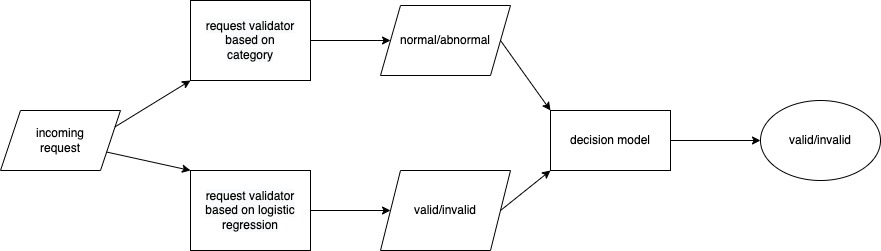
\includegraphics[width=\linewidth, height=10cm,keepaspectratio]{figures/architecture.jpg}
   \caption{Malicious request validator architecture}
\end{figure}
result: When two prediction is the same, the result is straight forward. When the logistic regression model decided that the request is malicious, but the CNN model predicted the request is nornal, the CNN is favored. Otherwise, the Regression model classified the request as valid but the CNN predicted as abnormal, we'll favor the Regression. The desicion model can be expressed in a decision table:


\begin{table}
\begin{center}
\begin{tabular}{||c c c ||} 
 \hline
 Regression & CNN & Result  \\ [0.5ex] 
 \hline\hline
 Valid & Normal & Valid \\ 
 
 Valid & Abnormal & Valid  \\

 Invalid & Normal & Valid  \\
 
 Invalid & Abnormal & Invalid  \\ [1ex] 
\hline
\end{tabular}
\end{center}
\caption{\label{demo-table}Table 4.1}
\end{table}

The CNN validator will run for a set period of time (usually one or two weeks) to collect the familiar category of incoming requests and assign a threshold (which can be the mean or maximum (if we are optimistic) distance between each request vector in the observing stage and the sum vector). The same will also happened with the Regression model. After that training phase, the module will run on 'active phase', parallel with the WAF. 
\begin{itemize}
    \item  To predict whether a request is malicious or not.
\end{itemize}
Our architecture is described in Figure 14 below, suggest a reasonable decision model for the combination of CNN and the Regression model
\begin{figure}[!h]
     \centering
     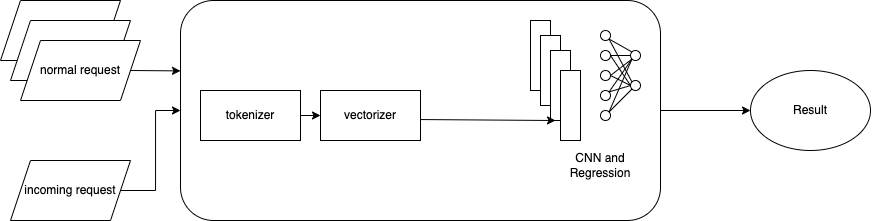
\includegraphics[width=\linewidth, height=10cm,keepaspectratio]{figures/architecture 2.drawio.png}
   \caption{Decision model for the combination of CNN and the Regression model}
\end{figure}
\newpage
The request is routed through the module, which predicts the category. The category of suspicious request is then compared with the common category. Then the Regression model will determined whether the request is good or bad, combining with the normal or abnormal status to decide the result. 
